\documentclass[11pt,a4paper]{article}

\usepackage[utf8x]{inputenc}
\usepackage[T1]{fontenc}

\usepackage{pdfpages}
\usepackage{palatino}
\usepackage{enumitem}
\usepackage{outlines} %support nested list
\usepackage{float}
\usepackage{framed}

\usepackage{desclist}

\setlist[itemize]{topsep=3pt,after=\vspace{.5\baselineskip}}
\usepackage[left=3cm,right=3cm,top=3cm,bottom=3cm]{geometry}
\setlength{\parskip}{2mm}


\def\blurb{\textsc{Université catholique de Louvain\\
  École polytechnique de Louvain\\
  Pôle d'ingénierie informatique}}
\def\clap#1{\hbox to 0pt{\hss #1\hss}}%
\def\ligne#1{%
  \hbox to \hsize{%
    \vbox{\centering #1}}}%
\def\haut#1#2#3{%
  \hbox to \hsize{%
    \rlap{\vtop{\raggedright #1}}%
    \hss
    \clap{\vbox{\vfill\centering #2\vfill}}%
    \hss
    \llap{\vtop{\raggedleft #3}}}}%
\begin{document}

\begin{titlepage}
\thispagestyle{empty}\vbox to 1\vsize{%
  \vss
  \vbox to 1\vsize{%
    \haut{\raisebox{-5mm}{
\includegraphics[width=2.5cm]{img/logo_ucl.pdf}}}{\blurb}{\raisebox{-5mm}{
\includegraphics[scale=0.20]{img/ingi_logo.png}}}
    \vfill
    \ligne{\Huge \textbf{\textsc{LINGI2251}}}
     \vspace{5mm}
    \ligne{\huge \textbf{\textsc{Software Engineering: Development Methods}}}
     \vspace{15mm}
    \ligne{\Large \textbf{\textsc{Assignment 2}}}
    \vspace{5mm}
    \ligne{\large{\textsc{12 april 2016}}}
    \vfill
    \vspace{5mm}
    \ligne{%
         \textsc{Alexandre Hauet\\Tanguy Vaessen} 
      }
      \vspace{5mm}
    }%
  \vss
  }
\end{titlepage}

%\tableofcontents

\section{Architectural Design}
\subsection{Hierarchical decomposition}

\begin{figure}[H]
 \centering
 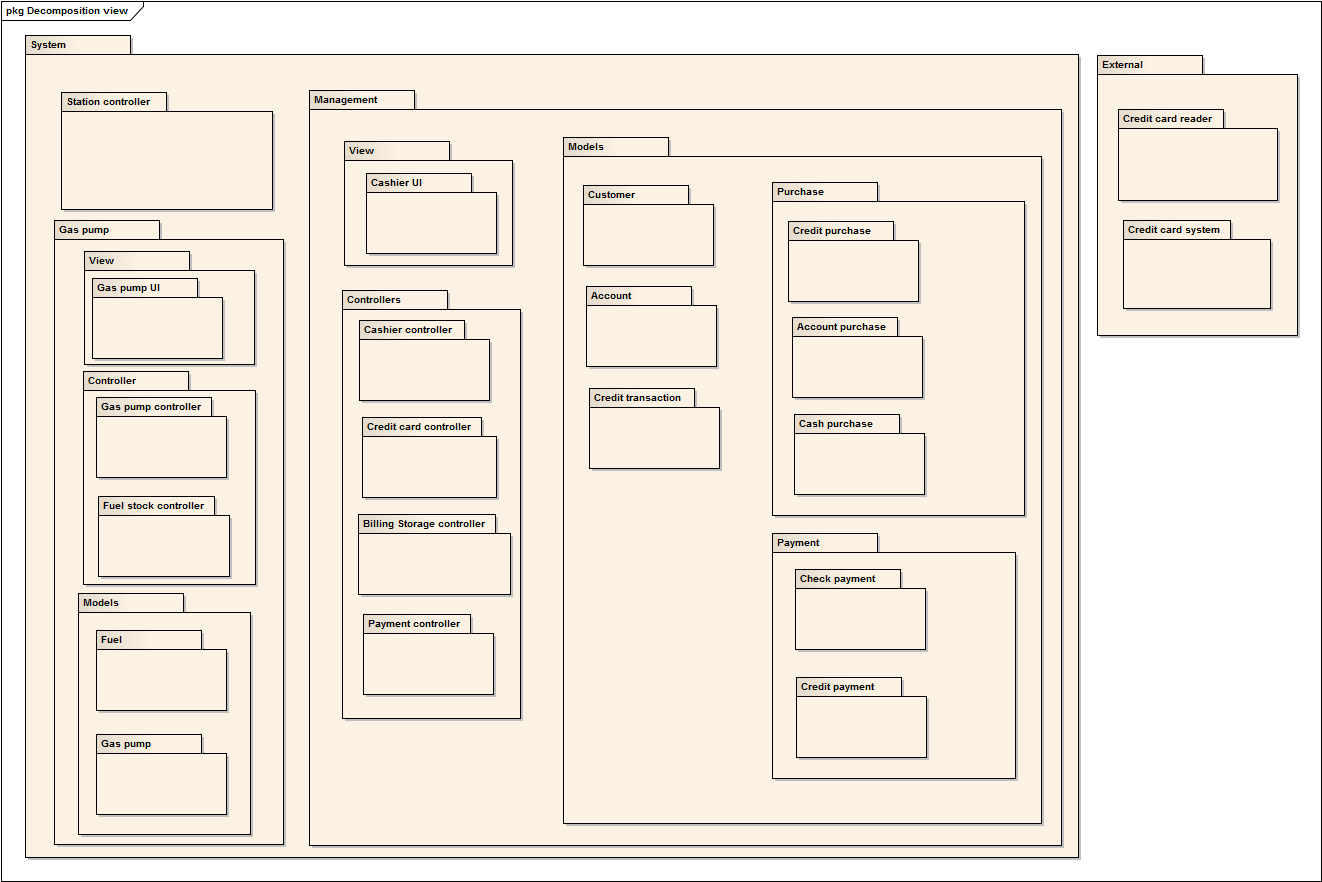
\includegraphics[width=\textwidth]{../DecompositionView.png} 
 \caption{Hierarchical decomposition}
 \label{fig:dep}
\end{figure}

\subsection{Roles and interactions of all components}

Our system is composed of three parts. The first is the station controller which control all the station. The second is the Gas Pump which is about the logistic of the pump. And finally, the Management part which allow to customers to pay or to manage the billing.

\subsubsection*{Station controller}

\subsubsection*{Gas Pump}
\begin{itemize}
\item{Gaz pump UI :} Interface with which the user interacts.
\item{Gaz pump controller :} Control the different interaction between the system (Station controler) and the different elements of the Gas pumps.
\item{Fuel stock controller :} Manage the stock of fuel of the station
\item{Fuel :} Represent a specific type of fuel
\item{Gaz pump :} Deliver the gaz to the costumers and compute the accounting. 
\end{itemize}
\subsubsection*{Management}
\begin{itemize}
\item{Cashier UI}
\item{Cashier controller}
\item{Credit card controller}
\item{Billing storage controller}
\item{Payement controller}
\item{Customer}
\item{Account}
\item{Credit transaction}
\item{Credit payment}
\item{Credit purchase}
\item{Account purchase}
\item{Cash purchase}
\end{itemize}

\section{Detailed Design}
\subsection{Class diagram}

\begin{figure}[H]
 \centering
 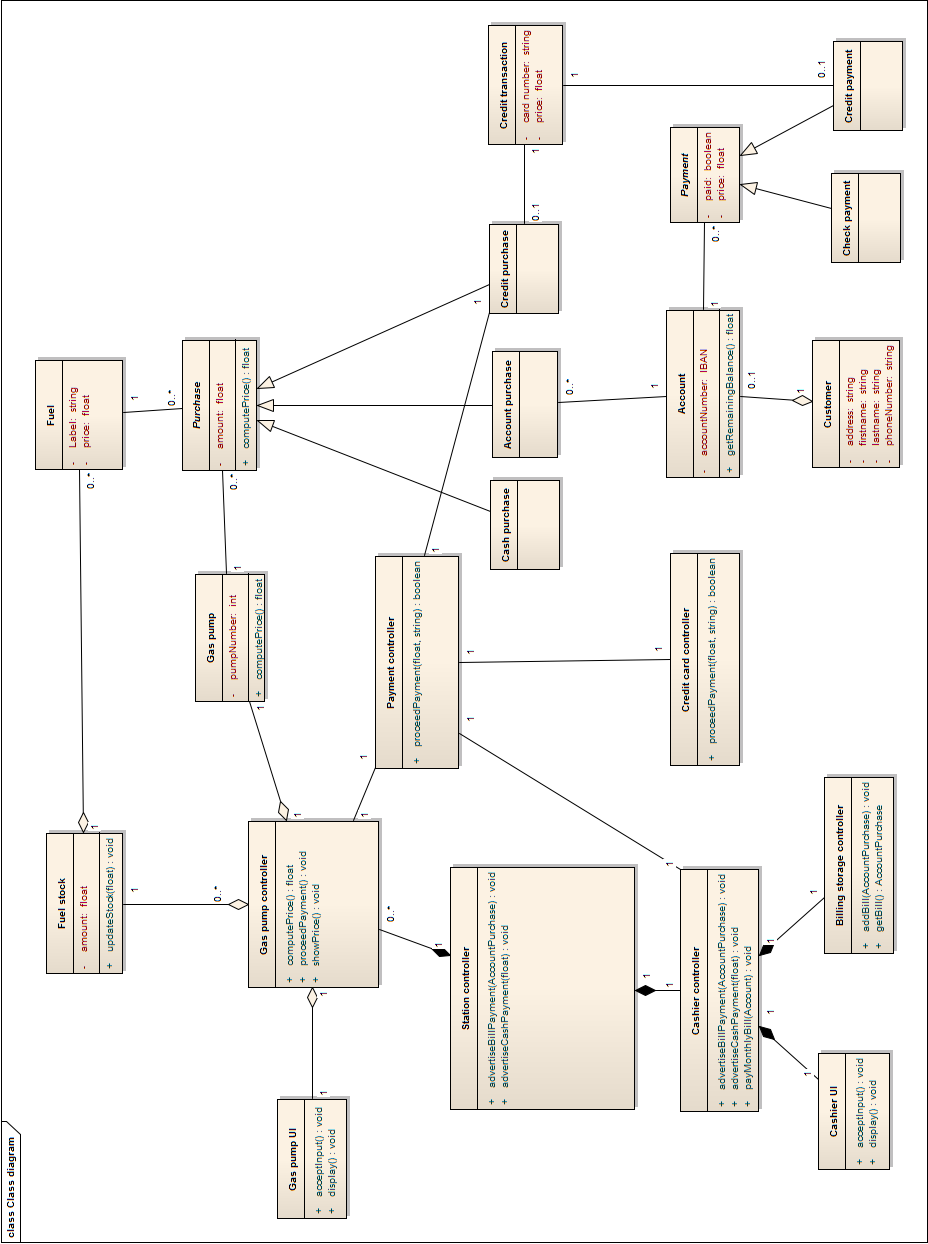
\includegraphics[width=\textwidth]{../ClassDiagram.png} 
 \caption{Class diagram}
 \label{fig:dep}
\end{figure}

\end{document}
